\chapter{The Compact Muon Solenoid}
\label{chap:detector}

\section{Introduction}

The Large Hadron Collider (LHC) at CERN is a 27\,km hadron accelerator and collider with a design centre-of-mass energy of 14\,TeV~\cite{LHC}.
Its purpose is to provide collisions sufficient in energy and number to precisely probe physics at the electroweak scale.
Four detectors, one of which is the Compact Muon Solenoid (CMS), are situated around the LHC ring.
CMS is a general-purpose detector designed to precisely measure a wide range of physics objects.
Together, the LHC and CMS facilitate a wide-ranging program of physics studies, from SM precision measurements to dark matter searches, 
and including the production and analysis of the Higgs boson.
This chapter will describe the design and operation of both the LHC and the CMS detector.

\section{The Large Hadron Collider}

The LHC is situated in the tunnel that previously housed the Large Electron Positron collider (LEP), 
around 100\,m below ground across the French-Swiss border near CERN.
It is the final machine in a series of accelerators which form the CERN accelerator complex; 
these  act as the injection system for the LHC.
The two counter-circulating beams cross at four interaction points, at each of which a detector is situated.
Directly opposite CMS is a second general purpose detector, ATLAS~\cite{ATLAS}, 
whose physics objectives are identical to those of CMS but with different design decisions.
The other two detectors, LHCb~\cite{LHCb} and ALICE~\cite{ALICE}, focus on flavour and heavy-ion physics respectively.
Whilst the LHC is capable of producing heavy ion collisions in addition to proton-proton collisions, 
the remainder of this section will be dedicated to its proton-proton operations.
A schematic of the full CERN accelerator complex and the LHC experiments is shown in Figure~\ref{fig:detector_CERNschematic}.
The operation of the LHC and the data it has accumulated so far is described in detail below.

\begin{figure}[h!]
  \centering
  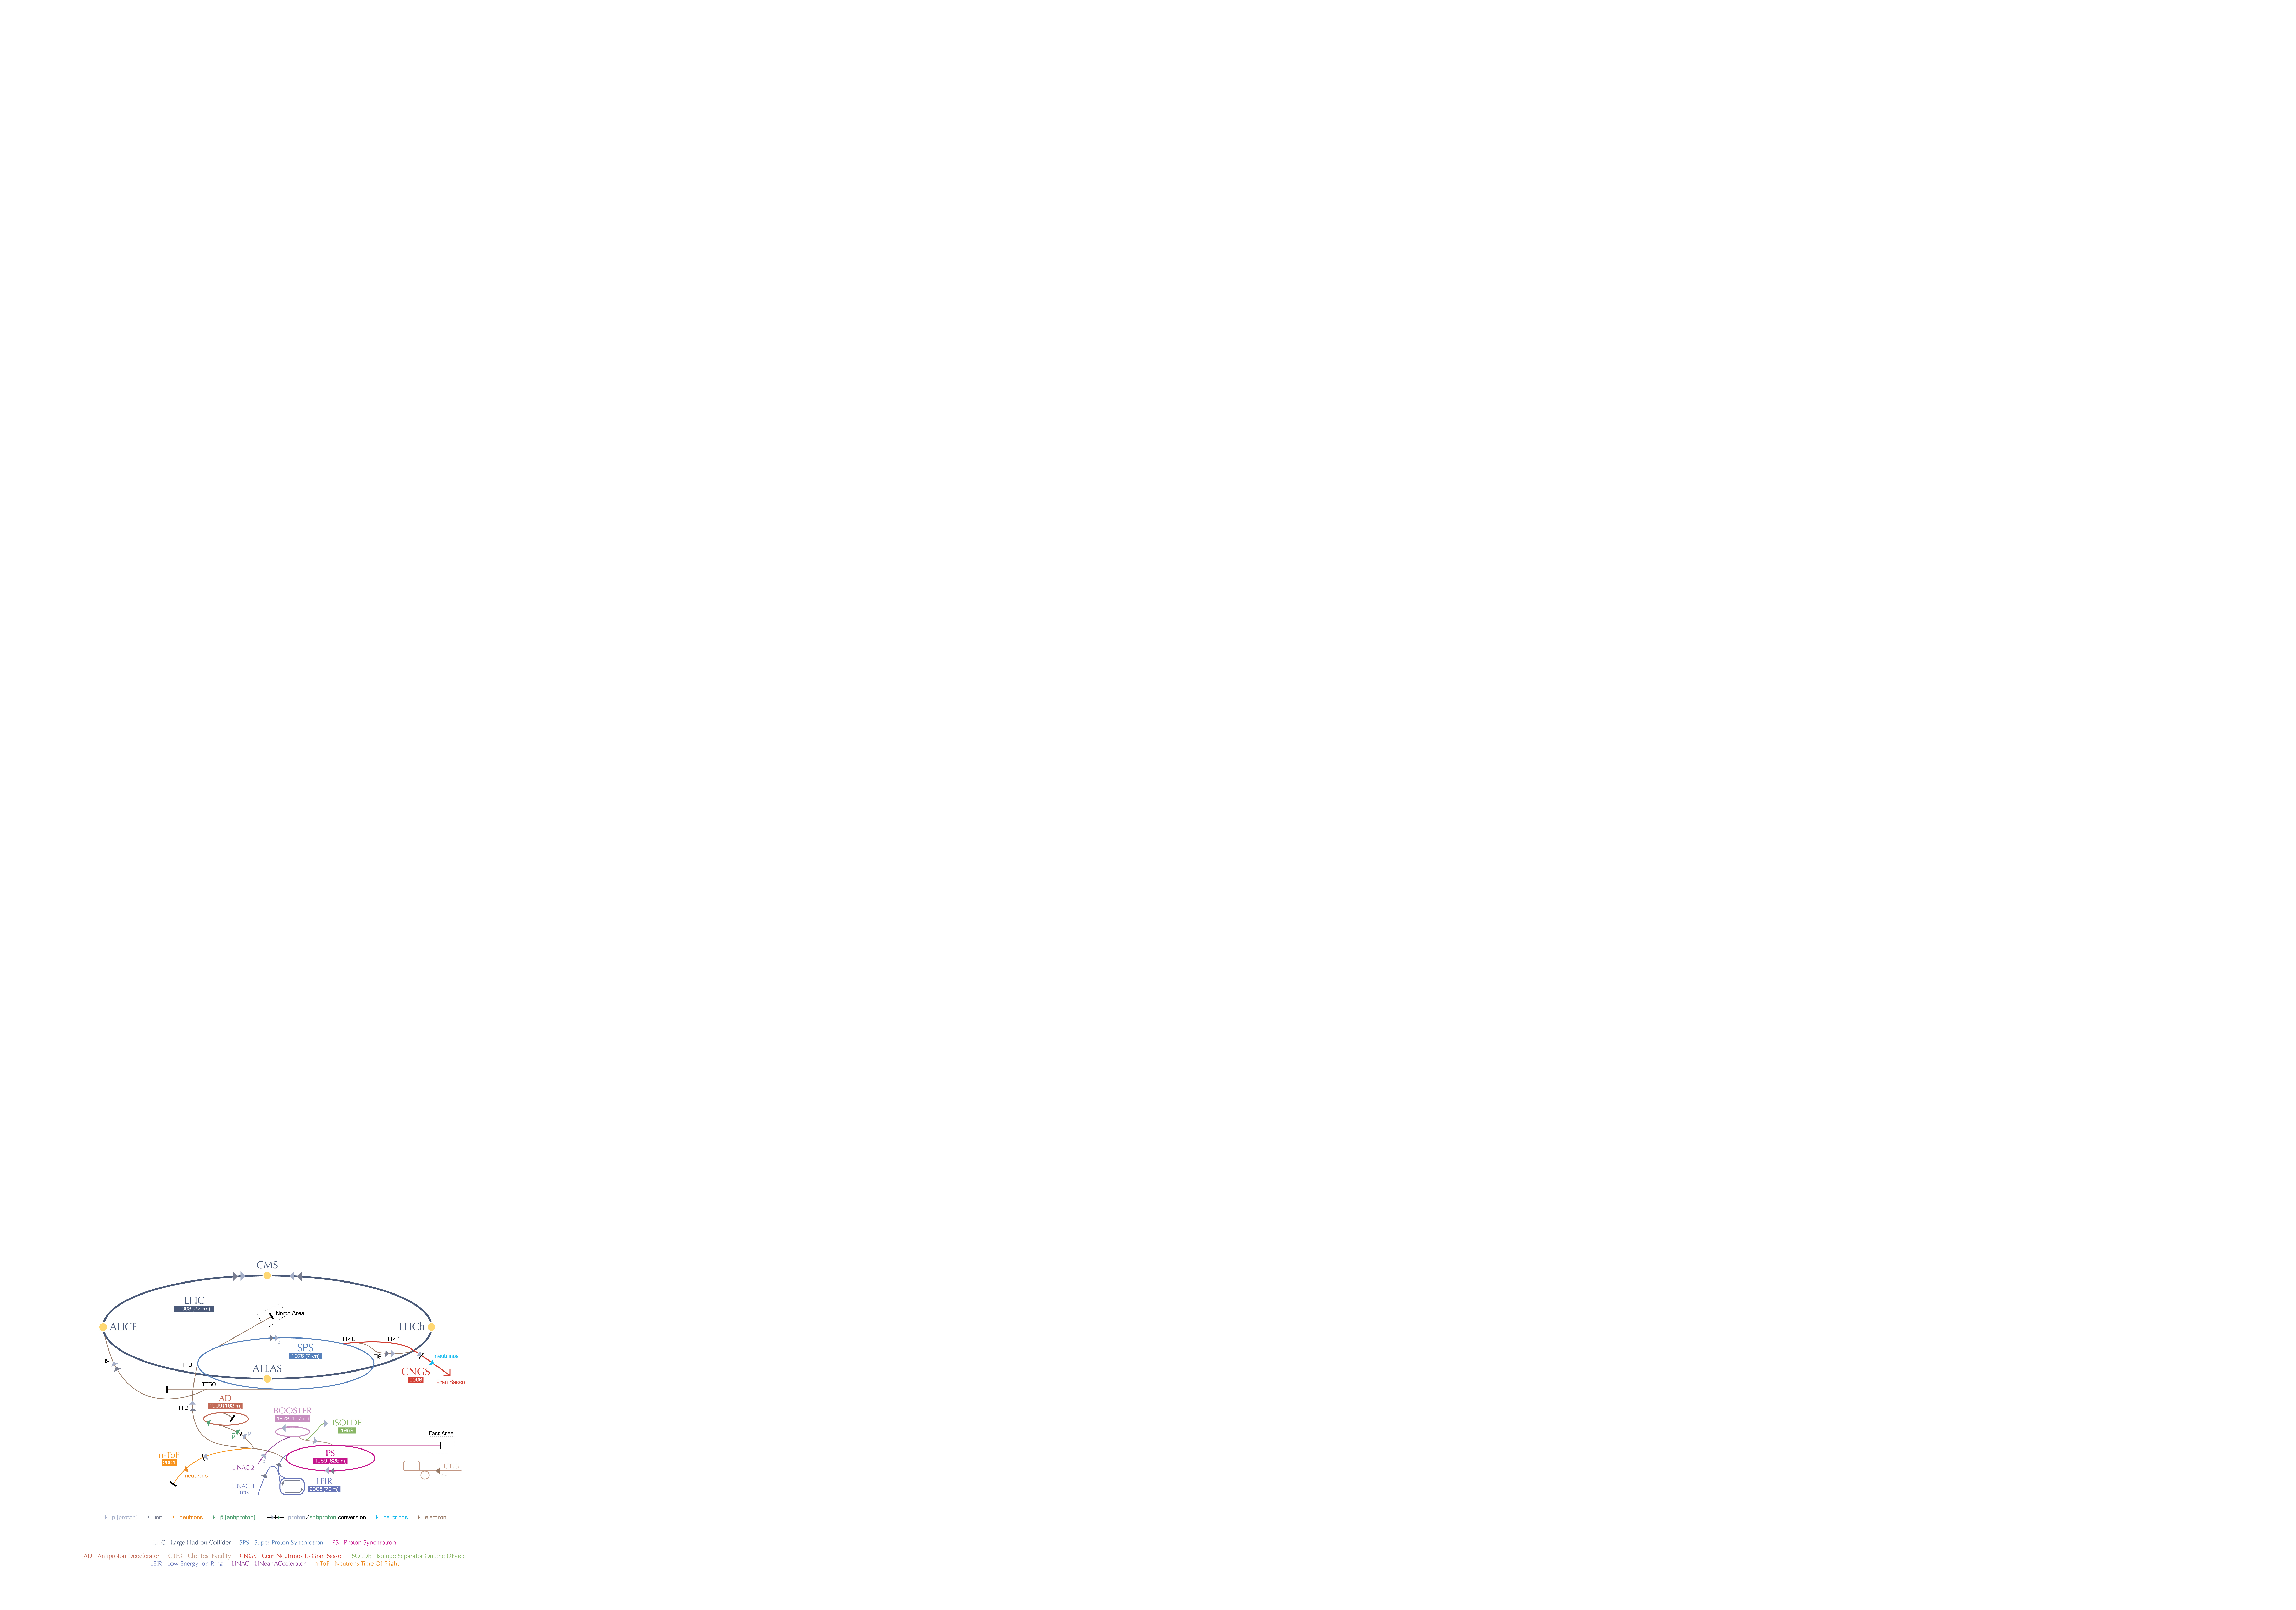
\includegraphics[width=\textwidth]{Figures/Detector/CERNschematic.pdf}
  \caption[The CERN accelerator complex.]
  {The LHC and its experiments within the CERN accelerator complex.
  Figure taken from Ref.~\cite{CERNcomplex}.}
  \label{fig:detector_CERNschematic}
\end{figure}

The LHC design parameters allow for proton-proton collisions to occur at a maximum centre-of-mass energy of 14\,TeV with an instantaneous luminosity of up to $10^{34}\,\textrm{cm}^{-2}\,\textrm{s}^{-1}$.
Prior to being injected into the LHC beam pipes, bunches of protons pass are accelerated in several stages. 
First, protons are obtained by stripping the electrons from hydrogen atoms using a strong electric field.
The protons produced are then accelerated up to an energy of 50 MeV by Linear Accelerator 2 (LINAC 2).
LINAC 2 leads into the Proton Synchrotron Booster (PSB), where they reach an energy of 1.4 GeV before passing into the Proton Synchrotron (PS).
Here the beam is accelerated up to 25 GeV before being transferred to the Super Proton Synchtroron (SPS).
The SPS is the last step before the protons enter the LHC itself at an energy of 540 GeV.
Therefore the LHC is responsible for the final acceleration from 540 GeV to the full energy.
Thus far, the energy reached for stable operation is 6.5\,TeV per beam; the full design energy is expected to be achieved in future.

The key components of the LHC are its 1232 main dipole magnets, 392 main quadrupole magnets and 16 radiofrequency (RF) cavities.
Superfluid helium cools the dipole magnets to 1.9K, at which temperature they produce the 8.3T magnetic field required to keep the beams in circular orbit.
Quadropole magnets are used principally to focus the beams near the interaction points, which increases the probability of a high-energy proton-proton collision.
The RF cavities deliver an accelerating field of 5MV/m at a frequency of 400MHz, and furthermore maintain the shape of the 2808 proton bunches per beam.
Collisions occur at the four interaction points, where bunches are induced to collide at a frequency of 25ns. 

The operation of the LHC to date has comprised two separate runs.
Run 1 commenced in 2010 with $\sqrt{s}$ = 7\,TeV, continuing into 2011 at the same centre-of-mass energy to give a total of 6.1\,\fb of data.
In 2012 this was increased to 8\,TeV, and a total of 23.3\,\fb of data were collected.
Analyses based upon this Run 1 dataset were able to discover the Higgs boson.
After a shutdown for upgrades to the machine, Run 2 ran from 2015 to 2018 at a constant 13\,TeV centre-of-mass energy.
The LHC was able to exceed its design luminosity in each of the years, eventually levelling the luminosity at $2\times10^{34}\,\textrm{cm}^{-2}\,\textrm{s}^{-1}$ for the majority of 2018 operations.
Figure \ref{fig:detector_Run1andRun2lumi} summarises the data collected in each year.
The latest \Hgg results on which this thesis is based have utilised the 2016 and 2017 datasets; 
plans for the final Run 2 result combining the 2016-2018 datasets are described in Chapter 9.

\begin{figure}[h!]
  \centering
  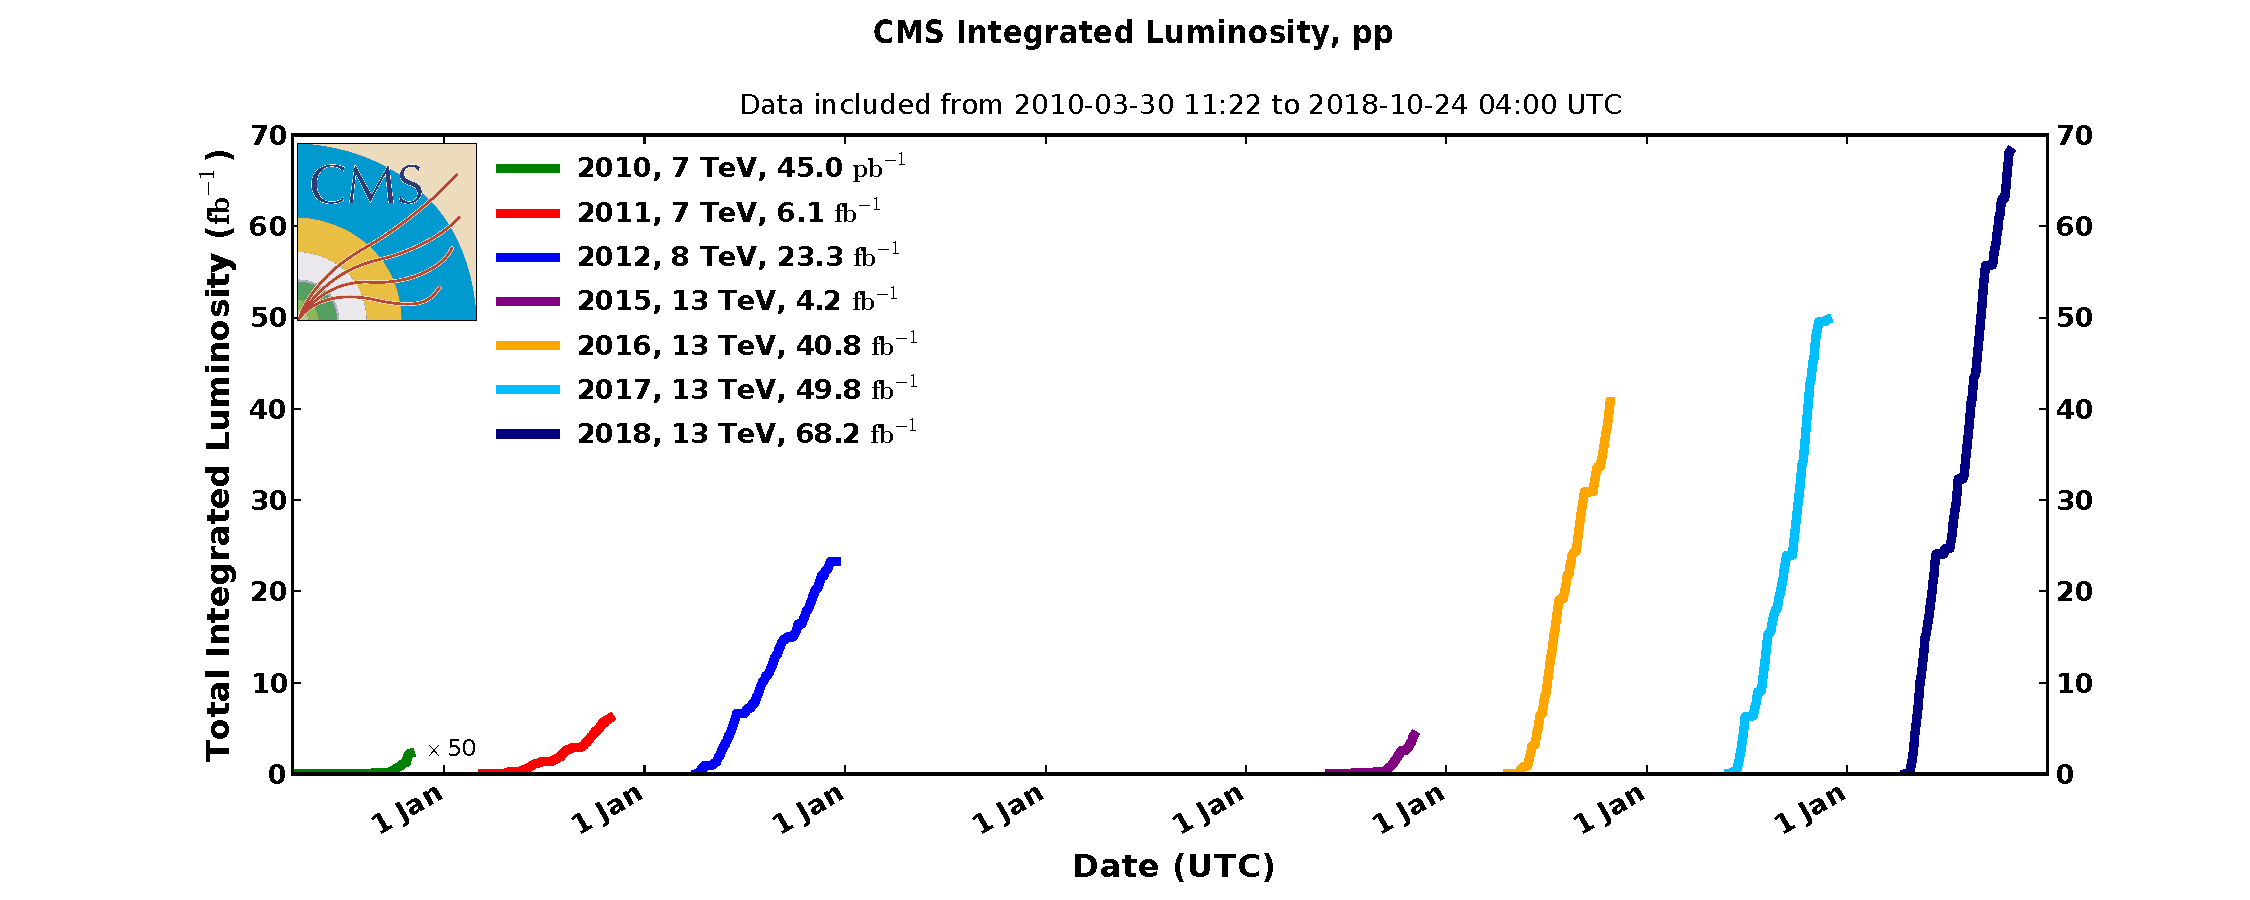
\includegraphics[width=\textwidth]{Figures/Detector/Run1andRun2lumi.pdf}
  \caption[LHC integrated luminosity and centre-of-mass energy per year.]
  {The integrated luminosity and centre-of-mass energy for each year of LHC operation.
  Figure taken from Ref.~\cite{CMSLumiPublic}.}
  \label{fig:detector_Run1andRun2lumi}
\end{figure}

\section{The CMS detector}

\subsection{Solenoid}
\subsection{Tracking}
\subsection{Electromagnetic calorimeter}
\subsection{Hadronic calorimeter}
\subsection{Muon system}
\subsection{Trigger system}
